\subsubsection{Simulation of the $x_I$ and $y_I$ Controllers}
The final design for the $x_I$ and $y_I$ translational controllers have been done. Only simulations of the $x_I$ controller is shown in the following, as the $y_I$ is identical. The simulations are both of the translational velocity controller and the positioning controller. The simulations which are presented are of the controller subjected to a step input reference signal and a corresponding simulation showing the related control action of the controller. 

In \autoref{fig:velocityControllersXY} the translational velocity controller, $\dot{x}_I$, is subjected to a step input reference signal of \SI{1}{m s^{-1}} at time \SI{0}{s}. This yields a settling time of \SI{6}{s}, with an error band of 5 percent, and an overshoot of 15 percent. In \autoref{fig:velocityControllersXYAction} the corresponding control action is shown.

\begin{minipage}{\linewidth}
    \begin{minipage}{0.5\linewidth}
        \begin{figure}[H]
            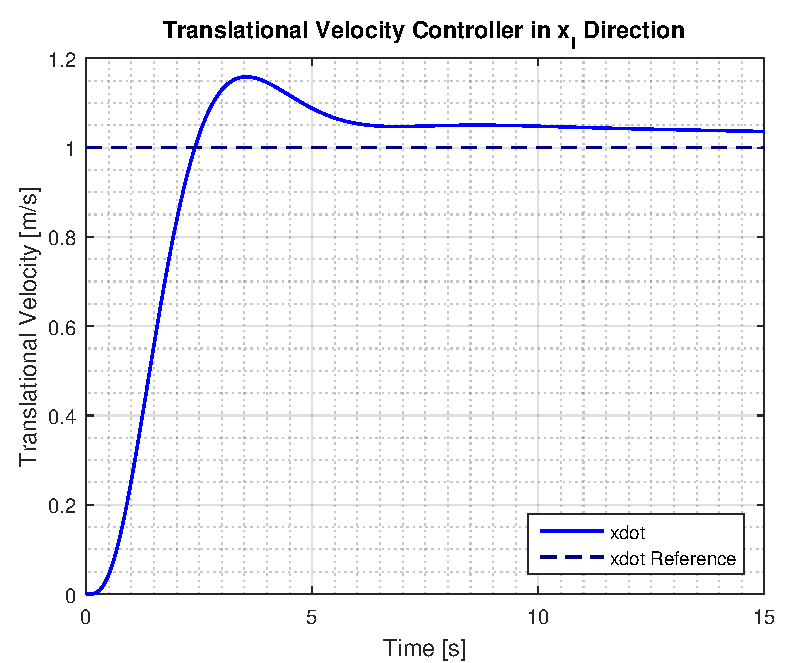
\includegraphics[scale=.5]{figures/velocityControllersXY}
            \centering			
            \captionof{figure}{A step response of the translational velocity controller, where the system is subjected to a step input reference signal of \SI{1}{m s^{-1}} in the $x_I$ direction at time \SI{0}{s}.}
            \label{fig:velocityControllersXY}
        \end{figure}
    \end{minipage}
    \hspace{0.03\linewidth}
    \begin{minipage}{0.5\linewidth}
        \begin{figure}[H]
            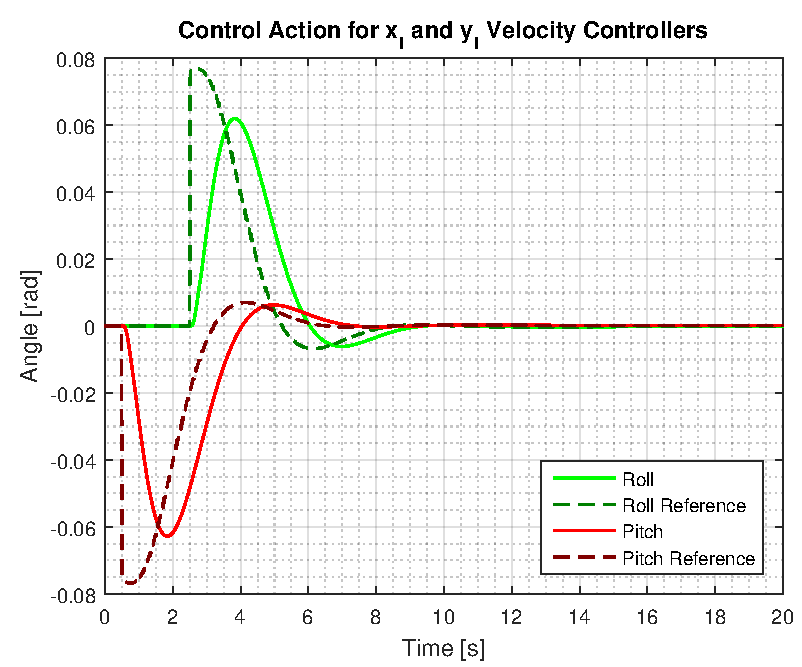
\includegraphics[scale=.5]{figures/velocityControllersXYAction}
            \centering
            \captionof{figure}{The performed control action to achieve the velocity response in \autoref{fig:velocityControllersXY}, together with the control action set by the controller.}
            \label{fig:velocityControllersXYAction}
        \end{figure}
    \end{minipage}
\end{minipage}

In \autoref{fig:positionControllersXY} the translational velocity controllers, $x_I$, is subjected to a step input reference signal of \SI{1}{m s^{-1}} at time \SI{0}{s}. Yielding a settling time of \SI{5}{s}, with an error band of 5 percent, and a overshoot of 2 percent. As the position controller are designed to have a closed loop bandwidth which is three times lower than the velocity bandwidth, a larger settling time is expected. However, as the overshoot is small compared to the velocity controller and the settling time has an error band, the settling time becomes lower.

\begin{minipage}{\linewidth}
    \begin{minipage}{0.46\linewidth}
        \begin{figure}[H]
            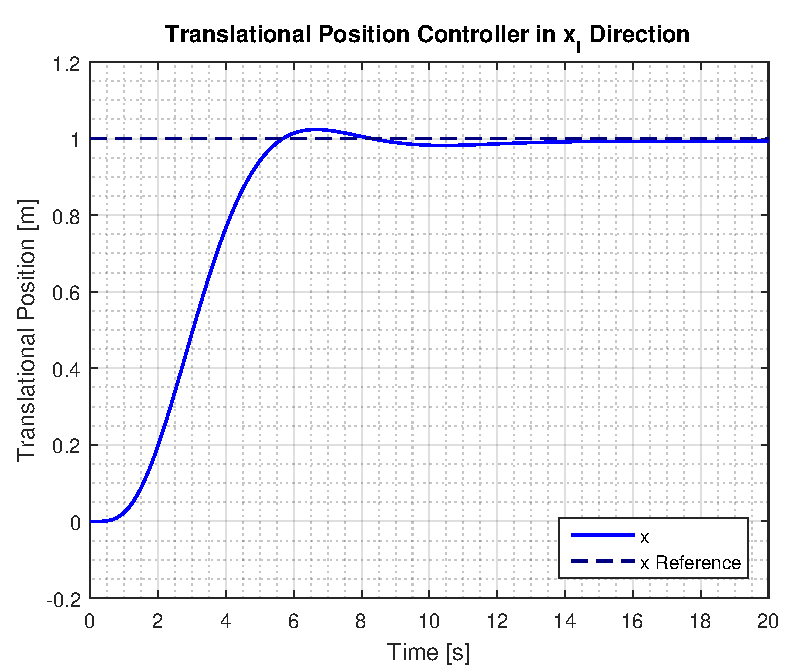
\includegraphics[scale=.6]{figures/positionControllersXY}
            \centering			
            \captionof{figure}{A step response of the position controller, where the system is subjected to a step input reference signal of \SI{1}{m} in the $x_I$ direction, at time \SI{0}{s}.}
            \label{fig:positionControllersXY}
        \end{figure}
    \end{minipage}
    \hspace{0.03\linewidth}
    \begin{minipage}{0.46\linewidth}
        \begin{figure}[H]
            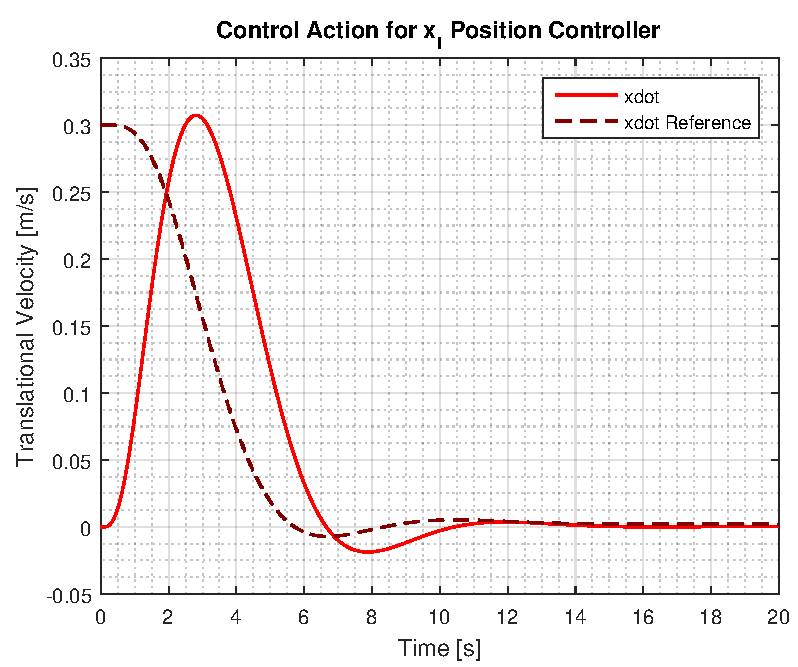
\includegraphics[scale=.6]{figures/positionControllersXYAction}
            \centering
            \captionof{figure}{The performed control action to achieve the position response in \autoref{fig:positionControllersXY}, together with the control action set by the controller.}
            \label{fig:positionControllersXYAction}
        \end{figure}
    \end{minipage}
\end{minipage}

The controller for the translational velocity and positioning in $x_I$ and $y_I$ direction have now been designed and simulated, the z controller can thereby be designed in the following section.
